\chapter{Level 1 : Mon premier jeu en Godot}

Pour ce premier contact avec Godot, nous allons tenter de réaliser un petit jeu sans prétention. Il s'agira d'un jeu où il faut attraper certains objets qui tombent du haut de l'écran, tout en évitant certains autres.

\section{Création du projet}

Quand vous lancez Godot, vous serez saluées par un écran comme celui de la figure \ref{lvl1-screen1}. Au premier lancement, il sera vide, mais vous verrez que bientôt il se remplira de tous les projets que vous aurez créés.

\begin{figure}
  \begin{center}
    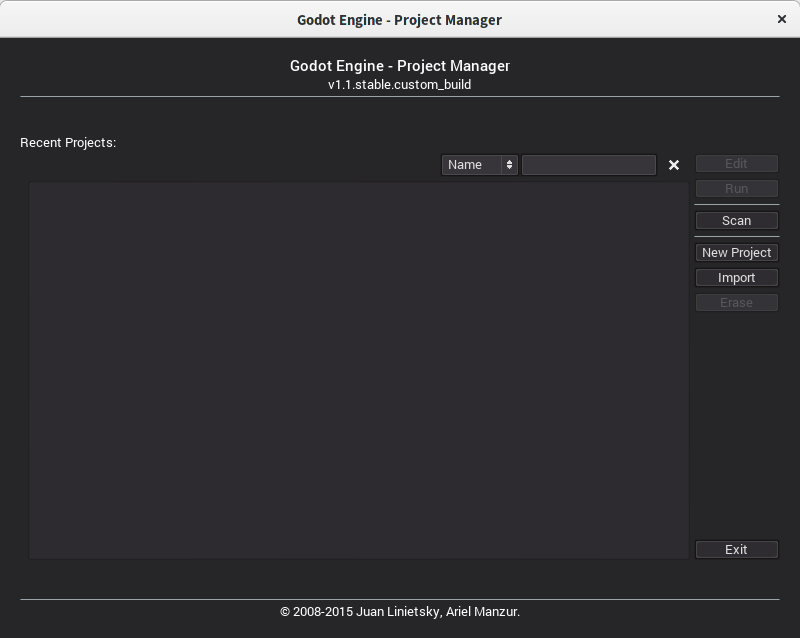
\includegraphics[width=12cm]{img/lvl1-screen1.png}
  \end{center}
  \caption{\label{lvl1-screen1} L'écran de sélection de projets de Godot, sa façon de vous dire bonjour.}
\end{figure}

Le bouton qui nous intéresse plus particulièrement est le bouton \emph{New Project}, qui va nous permettre de... créer un nouveau projet (qui l'eut crû). Vous verrez une popup s'ouvrir, comme sur la figure \ref{lvl1-screen2}.

\begin{figure}
  \begin{center}
    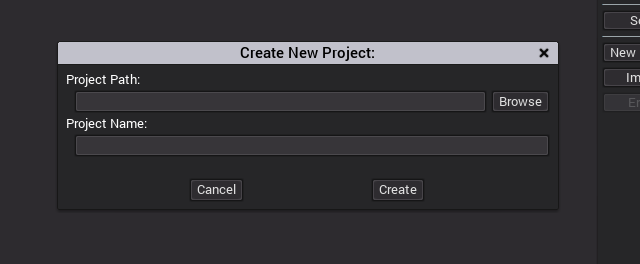
\includegraphics[width=10cm]{img/lvl1-screen2.png}
  \end{center}
  \caption{\label{lvl1-screen2} Un nouveau projet ! Sentez-vous l'excitation qui monte, la hype qui se profile ? Non ? Ah bon...}
\end{figure}

En utilisant le bouton \emph{Browse}, vous pourrez naviguer jusqu'à trouver un endroit parfait pour votre projet. Tous les fichiers du projet seront stockés dans ce dossier. En plus, Godot vous encourage à donner un nom intelligent à votre dossier: par défaut, le nom du dossier sera également le nom du projet. Dans un énorme élan de créativité, j'ai décidé d'appeler mon dossier \codeintext{FallingThings}, d'après le principe de notre jeu.

Une fois la boite de dialogue remplie et validée, vous aurez l'insigne honneur de voir votre nouveau projet apparaître dans la fenêtre de sélection de projets (voir figure \ref{lvl1-screen3}).

\begin{figure}
  \begin{center}
    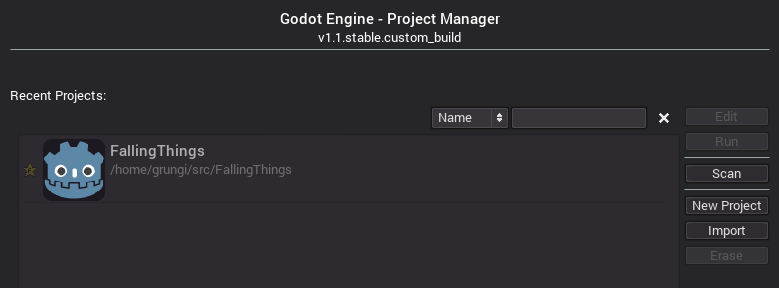
\includegraphics[width=12cm]{img/lvl1-screen3.png}
  \end{center}
  \caption{\label{lvl1-screen3} Et voilà, le projet est maintenant prêt à être ouvert, et le travail va pouvoir commencer.}
\end{figure}

Les choses sérieuses peuvent commencer !

\section{Le Nouveau Monde}

Tels des exploratrices devant les côtes d'une île inconnue, vous avez ouvert votre projet, et vous vous êtes retrouvées devant un écran relativement intimidant. Pas très loin de celui de la figure \ref{lvl1-screen4}.

\begin{figure}
  \begin{center}
    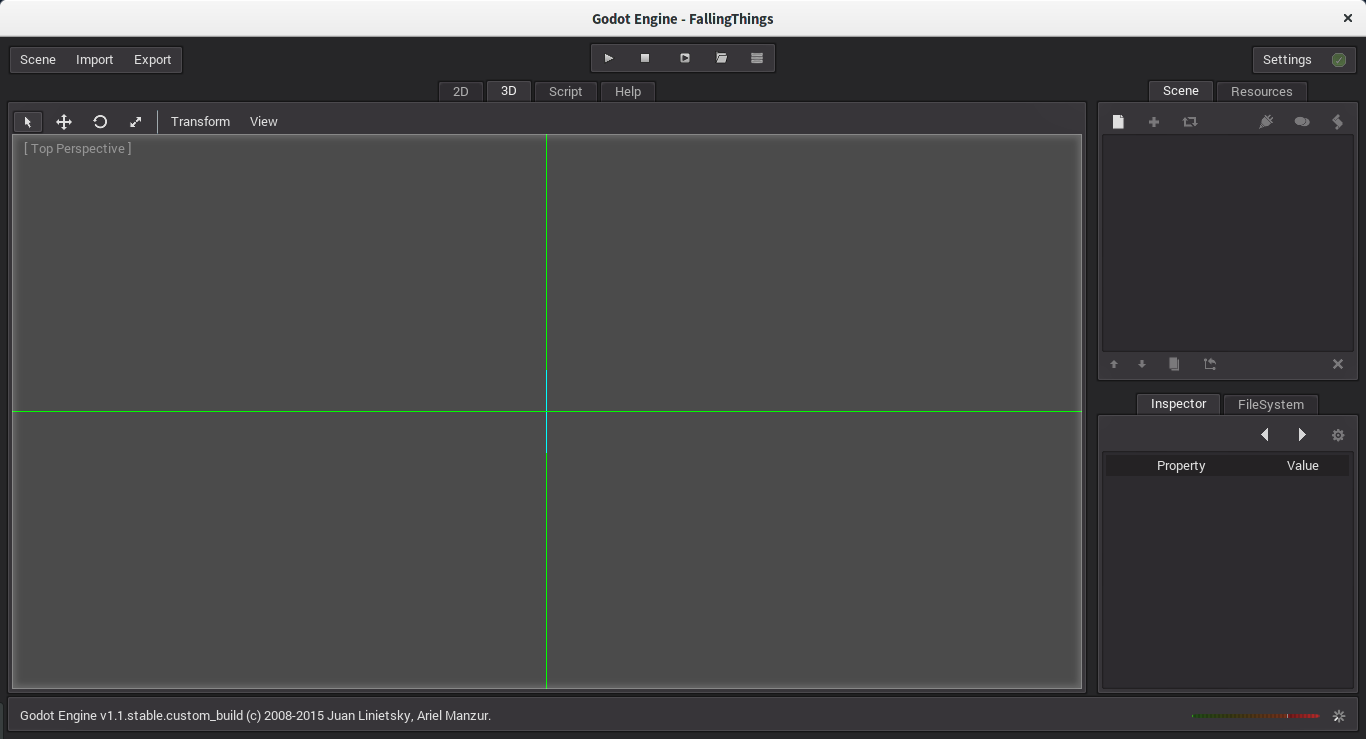
\includegraphics[width=12cm]{img/lvl1-screen4.png}
  \end{center}
  \caption{\label{lvl1-screen4} Des icones, des boutons, des onglets... Bienvenue dans Godot !}
\end{figure}

Pas de panique cependant, c'est plus simple qu'il n'y parait. L'écran est divisé 5 zones principales.

\begin{description}
\item[En haut] : On retrouve des menus, que nous explorerons petit à petit, une barre de boutons qui permettent de lancer le jeu, le stopper, lancer une \emph{scène}, et un bouton sur la droite permettant de modifier certains paramètres de l'éditeur de Godot.
\item[Au centre] : La majeure partie de l'écran est occupée par la zone de travail principal de Godot. Comme un navigateur, elle se présente sous la forme de plusieurs onglets. Le premier de ceux-ci offre une vue 2D de l'application (nous allons souvent l'utiliser), le deuxième sert dans le cadre de projets 3D, le troisième sert à éditer les scripts (le code), et le dernier vous offre l'aide de Godot, bien utile à avoir sous la main.
\item[A droite, en haut] : Vous trouverez là la hiérarchie des \emph{noeuds} présents dans la \emph{scène} en cours. Ce charabia deviendra plus intelligible quand nous parlerons de comment Godot organise les éléments des projets un peu plus loin. Mais retenez que c'est là que vous trouverez les différents éléments qui sont actuellement dans votre jeu. Le second onglet, \emph{Resources}, vous montrera les différentes sources de données (textures, sprites, fichiers sons, ...) qui seront utilisées dans le projet. Nous y reviendrons également plus tard.
\item[A droite, en bas] : Là où l'onglet \emph{Scene} ci-dessus vous montrait la liste des éléments de la \emph{scène}, l'onglet \emph{Inspector} vous renseigne les propriétés de l'objet actuellement sélectionné. Vous pourrez l'utiliser pour définir un grand nombre d'options pour chaque objet. A ses côtés, l'onglet \emph{FileSystem} vous montre simplement un navigateur qui vous permet de parcourir l'arborescence des dossiers de votre projet.
\item[En bas] : Tout en bas de la fenêtre, vous trouverez une barre de statut, qui vous montrera les sorties générées par les commandes que vous utiliserez ou par votre jeu. En cliquant dessus, vous pourrez faire apparaître une zone plus conséquente où vous pourrez voir plus de texte.
\end{description}

Voilà, maintenant que vous êtes familiarisées avec l'organisation générale de l'interface du moteur, il est temps de voir comment utiliser tout cela.

\section{Le \emph{noeud} du problème}


